\section{Results from Prior NSF Support}
\label{sec:prior}

%%% XXX Everyone, please check if all of your grants are listed.
%%% XXX Greg: any Auger-only NSF support?
%%%
In the past five years the research activities of the UNL HEP group have been supported by these NSF grants: 
% CMS ops grant, 2012-2016
PHY-1120138, ``U.S. CMS Operations at the LHC,'' PI Marlow (Princeton), \$43,794,718, 1/1/12-12/31/16; 
% CMS ops grant, 2012-2016
PHY-1624356, ``U.S. CMS Operations at the LHC,'' PI Marlow (Princeton), \$26,249,987 to date, 1/1/17-12/31/21; 
% Pixels, 2007-2014
OISE-0730173, ``PIRE: Collaborative research with the Paul Scherrer Institute and Eidgenoessische Technische Hochschule on Advanced Pixel Silicon Detectors for the CMS detector,'' PIs Bean (KU), Dominguez {\it et al.}, \$2,677,658, 10/1/07-9/30/14; 
% Computing AAA, 2011-2016
PHY-1104664, ``Collaborative Research: Any Data, Anytime, Anywhere,'' PI Bloom, \$710,336, 9/15/11-2/29/16;
% DASPOS
PHY-1247316, ``Data and Software Preservation for Open Science," PI Hildreth (UND) {\it et al.}, \$2,065,046, 9/15/12-8/31/17;
% Pixels upgrade, 2014-2019
PHY-1343486, ``U.S. CMS Phase-1 Upgrades,'' PIs Bean (KU), Dominguez {\it et al.}, \$9,355,988, 6/15/14-5/31/19;
% UNL HEP group grant 2013-2016
PHY-1306040, ``Experimental Particle Physics at the Energy and Cosmic Frontiers,'' PIs Bloom, Claes, Dominguez, Kravchenko and Snow, \$2,055,000, 9/1/13-8/31/16;
% CROP grant 2013-2016
DRL-1311782, ``Strategies: Action at a Distance ITEST,'' PIs: Claes, Snow, {\it et al.}, \$550,000, 08/01/13-07/31/16;
% Current HEP base grant 2016-19
PHY-1607202, ``Particle Physics Research with the CMS Experiment at the LHC," PIs Kravchenko, Bloom, Claes, Dominguez and Snow, \$2,070,000, 8/1/16-7/31/19.
(All award amounts are those of the total award; where non-UNL PI's are named, UNL received a sub-award.)


\subsection{Intellectual Merit}

\paragraph{CMS}

The UNL HEP group has made significant contributions to the CMS experiment across a broad range of activities: physics measurements, construction, operations, and preparations for upgrades. The activities completed span a wide array of topics for a mid-sized university group and have made a broad impact on the CMS research program.

%
% Early data 
%
Standard model (SM) measurements were the focus of the group at the start of LHC in 2010 and 2011. Kravchenko worked within the CMS Vector Boson Task Force on one of the first physics papers from the CMS experiment, the measurement of the inclusive W and Z production cross section at 7\TeV~\cite{bib:firstWandZxsec}. Bloom, Dominguez, former postdoc Helena Malbouisson, graduate student Jason Keller and undergraduate Maxwell Gregoire led a joint effort with Cornell, Maryland and CERN for a first measurement of the $t\bar t$ production cross section, using soft muons to identify $b$-quark jets from $t\bar t$ decay~\cite{bib:smtxsec}. This channel was an important cross check of the measurement performed with displaced-vertex tags. In 2013, Keller, guided by Claes, completed his work demonstrating that soft electron tagging can be effectively used for a $t\bar t$ production cross section measurement, and defended it as his PhD thesis~\cite{bib:Keller-thesis}. 

These analyses helped develop analysis tools such as $b$ tagging that were used throughout CMS in later analyses.  As CMS continued to accumulate large datasets at 7 and 8\TeV, the group moved to performing high precision SM measurements, Higgs physics and new physics searches.

%
% SM precision and other measurements
%

Kravchenko, former postdoc Jamila Bashir Butt and graduate students Ekaterina Avdeeva and Rami Kamalieddin studied the Drell-Yan process, producing papers on differential cross section measurements with respect to the invariant mass and rapidity of the mediating $Z/\gamma^*$ at 7\TeV~\cite{bib:DY7TeV} and 8\TeV~\cite{bib:DY8TeV}. 

Since 2012, UNL has led the effort on single top physics in CMS. Postdoc Rebeca Gonzalez Suarez served as a co-convener of the CMS Single Top group in 2012-14, overseeing all CMS analyses on the topic. She was also one of the primary authors on several of the measurements in this area, including the analyses of the single top production in the s- and t-channels, searches for flavor changing neutral currents in events with single top, and others \cite{bib:single-top-papers}.

%
%   Higgs related work
%

The group has made a significant contribution to the Higgs boson discovery and measurements of its properties at CMS. Kravchenko and Gonzalez Suarez were the primary authors of a search for Higgs production associated with a $Z$ boson and the subsequent decay of the $ZH$ system into the $3\ell+2\text{jets}+1\nu$ final state, the results of which were published in the CMS legacy paper on $H\rightarrow WW$ studies of Run~1~\cite{bib:HWWlegacy}. Kravchenko and Gonzalez Suarez have also completed a thorough investigation of different spin-parity hypotheses for the newly discovered boson with $H\rightarrow VV$, where the UNL group in collaboration with MIT covered the $H\rightarrow WW$ half of the paper~\cite{bib:higgs-spin-parity}.

Bloom and graduate student Daniel Knowlton were leaders of the effort to search for the anomalous production of single top quarks in association with Higgs bosons ($tHq$), using the $H \to b\bar{b}$ decay mode~\cite{bib:tHqbbPAS}. They developed a data-driven method to estimate the $t\bar{t}$ background that dominates the event sample.  Bloom then co-edited the paper that combines that result with three others that use different Higgs decay modes~\cite{bib:tHqpaper}.  This is the only search ever for the $tHq$ production mechanism.

Dominguez and Bloom supervised the PhD thesis work of Rachel Bartek, who was then a visiting student from UC Riverside and is now a postdoc with our group.  She performed a search for $ZH$ production with $Z \to \tau\tau \to e\mu$ and $H \to b{\bar{b}}$, as a complement to searches with other $Z$ decay modes.  The search proved challenging because of the significant background from $t\bar{t}$ production, but Bartek's measured upper limit on the process was in good agreement with expectations, demonstrating a good modeling of the $t\bar{t}$ rate in this area of phase space~\cite{bib:Bartekthesis}.

Claes and postdoc Suvadeep Bose working with several other collaborators have performed the first search for lepton-flavor violating Higgs decays in CMS. This direct search was conducted for the $H\rightarrow \tau\mu$ signature, and is an order of magnitude more sensitive than prior indirect searches. No lepton-flavor violating Higgs decays were found in the analysis and limits on the branching ratio for this final state have been set, as reported in the resulting paper~\cite{bib:higgs-LFV}.

%
% Rare decays, new physics
%

Former postdoc Jose Lazo-Flores worked on the first observation of the decay $B_s \to \mu\mu$, and was the only U.S.-supported CMS physicist on this uniquely sensitive-to-new-physics study. He leveraged his residency at the Paul Scherrer Institute (PSI) under the Partnerships in International Research and Education (PIRE) program to work with staff there on this search.  The measured rate was consistent with that predicted by the standard model, which puts constraints on many models of new physics~\cite{bib:Bsmumu}.

Claes and Bose pursued searches for new physics looking for quark compositness, quark contact interactions, and extra spatial dimensions in CMS dijet events employing an angular analysis technique. No deviations from the standard model have been found and limits on the related new physics parameters were published~\cite{bib:quark-compositness-etc}.

Several measurements ongoing at UNL are expected to be published within less than a year. The most advanced are a search for the anomalous triple gauge coupling in $W\gamma$ production with 8\TeV CMS data by Kravchenko and Avdeeva (planned to be Avdeeva's PhD thesis), where the measurement itself is completed and about to undergo collaboration review, and a study of the Higgs production in association with a $t\bar{t}$ pair with a multilepton signature based on the Run~2 13\TeV CMS data that is expected to produce first public results in 2016.  Postdoc Bartek recently submitted for publication an analysis looking for the production in 8\TeV data of excited bottom quarks, an exotic form of matter predicted by many theories beyond the standard model~\cite{bib:bstar}. 

%
% Service, reconstruction, etc
%

The group's work on physics measurements is grounded in strong efforts on object reconstruction and identification.  During LHC Run~1, the UNL group had responsibility for supporting $b$-tagging algorithms and Dominguez was the $b$-tag co-convener at the LHC Physics Center (LPC).  Keller and Knowlton validated and certified $b$-tagging code in CMS software releases.  Bloom co-edited a lengthy paper documenting the algorithms and their performance~\cite{bib:btagperformance}.

Over the last four years, Kravchenko has played an important role in the CMS $e$-$\gamma$ (EGM) Physics Object Group. Through 2012 and 2013, Kravchenko was an EGM Object Expert for the Standard Model Physics (SMP) group of CMS, overseeing all usage of electrons in the SMP measurements and serving as the EGM-SMP liaison. Since 2014, Kravchenko has been the co-convener of the Electron and Photon Identification EGM subgroup, responsible for development and calibration of all aspects of identification for these particles. He also was responsible for computing electron reconstruction and identification scale factors in Run 1 \cite{bib:EGM-Run1-SF} that have been used across numerous measurements from CMS. In 2015, Kravchenko was one of the two lead developers of the electron and photon identification software framework in CMS software. In addition to the overall ID framework, Kravchenko has guided Kamalieddin on development of specific electron selection criteria sets for different data and MC sets for Run 2.  

Working with Dominguez, postdoc Bose was a key contributor to the understanding of the tracking and vertexing performance of the CMS pixel detector.  The pixel detector, which seeds the offline reconstruction of tracks, is also used as a standalone fast tracking detector in the high level trigger and is crucial for precise vertexing near the interaction point.  Understanding the performance of the pixel detector's reconstruction efficiency, resolution and fake rate are necessary components for the CMS physics program.  These results were documented in a recent article~\cite{bib:trackperf}. 

Postdoc Frank Meier became convener of the CMS tracker alignment group in 2013.  The tracker must be aligned to a fine degree to reach sub-ten-micron space point measurement precision.  Meier led the effort to achieve an incredible 1-2 micron precision alignment of the individual components of the silicon tracker~\cite{bib:alignment}.  Avdeeva worked with Meier first on aligning the tracker using cosmic rays during the period before proton collisions and later with collision data at the start of Run~2.

In computing, Bloom and Dominguez have overseen the operation of UNL’s Tier-2 computing center, along with David Swanson of UNL’s Holland Computing Center (HCC). This center is one of seven in the US and fifty in all of CMS. The center is supported by two full-time staff members, and currently operates about 4600 batch slots and hosts 1.5~PB of data. The Nebraska center is routinely ranked among the best in all of CMS in just about every metric. Bloom also served as the US CMS Level 2 manager for the Tier-2 program, CMS-wide co-coordinator for all Tier-2 centers, and U.S. CMS Software and Computing deputy manager, where he helped oversee all US CMS software and computing activities.  In January 2015, he was promoted to Software and Computing Operations Manager for the U.S. CMS Operations Program, a role of major responsibility in the experiment.  UNL was the host institution for Sudhir Malik, who served as the CMS Level 2 manager for computing user support, until his departure in August 2014, and continues to host computing professional Rob Snihur, who is co-responsible for US Tier-3 facility support.

Members of the UNL computing staff led the NSF-funded ``Any Data, Anytime, Anywhere'' (AAA) project, which has made data access over the wide-area network transparent and efficient. This technology has been adopted by CMS, leading to changes in the experiment's computing model and revolutionizing data access for other data-intensive, high-throughput applications~\cite{bib:AAA}.

Dominguez led the international CMS effort to plan a first upgrade (``Phase-1 Upgrade'') of the pixel detector. This proceeded his roles as the U.S. CMS Forward Pixel Detector Deputy and Project Manager, and the international CMS Tracker Project Manager Deputy.  He edited the resulting Technical Design Report~\cite{bib:pixTDR}.  The Phase-1 Upgrade of the Forward Pixel Detector was subsequently organized by Dominguez in the U.S. and became part of Cooperative Agreement between the NSF and UNL to fund all aspects of the CMS Phase-1 upgrade, of which he is the PI and UNL is the lead institution.  The goal of the Phase-1 Upgrades is to preserve the ability to reconstruct all the standard model objects and missing energy at higher luminosity than the original design through upgrades to the pixel detector, hadron calorimeter and Level-1 trigger.  It aims to achieve similar or better efficiency, resolution, trigger thresholds and background rejection at 13\TeV with more than 50 simultaneous interactions (``pileup'') than CMS had at 8\TeV with less than 20 pileup.  The UNL group's main role in the construction of these upgrades is the design and fabrication of half of all the forward pixel detector modules.  
\begin{figure}
\centering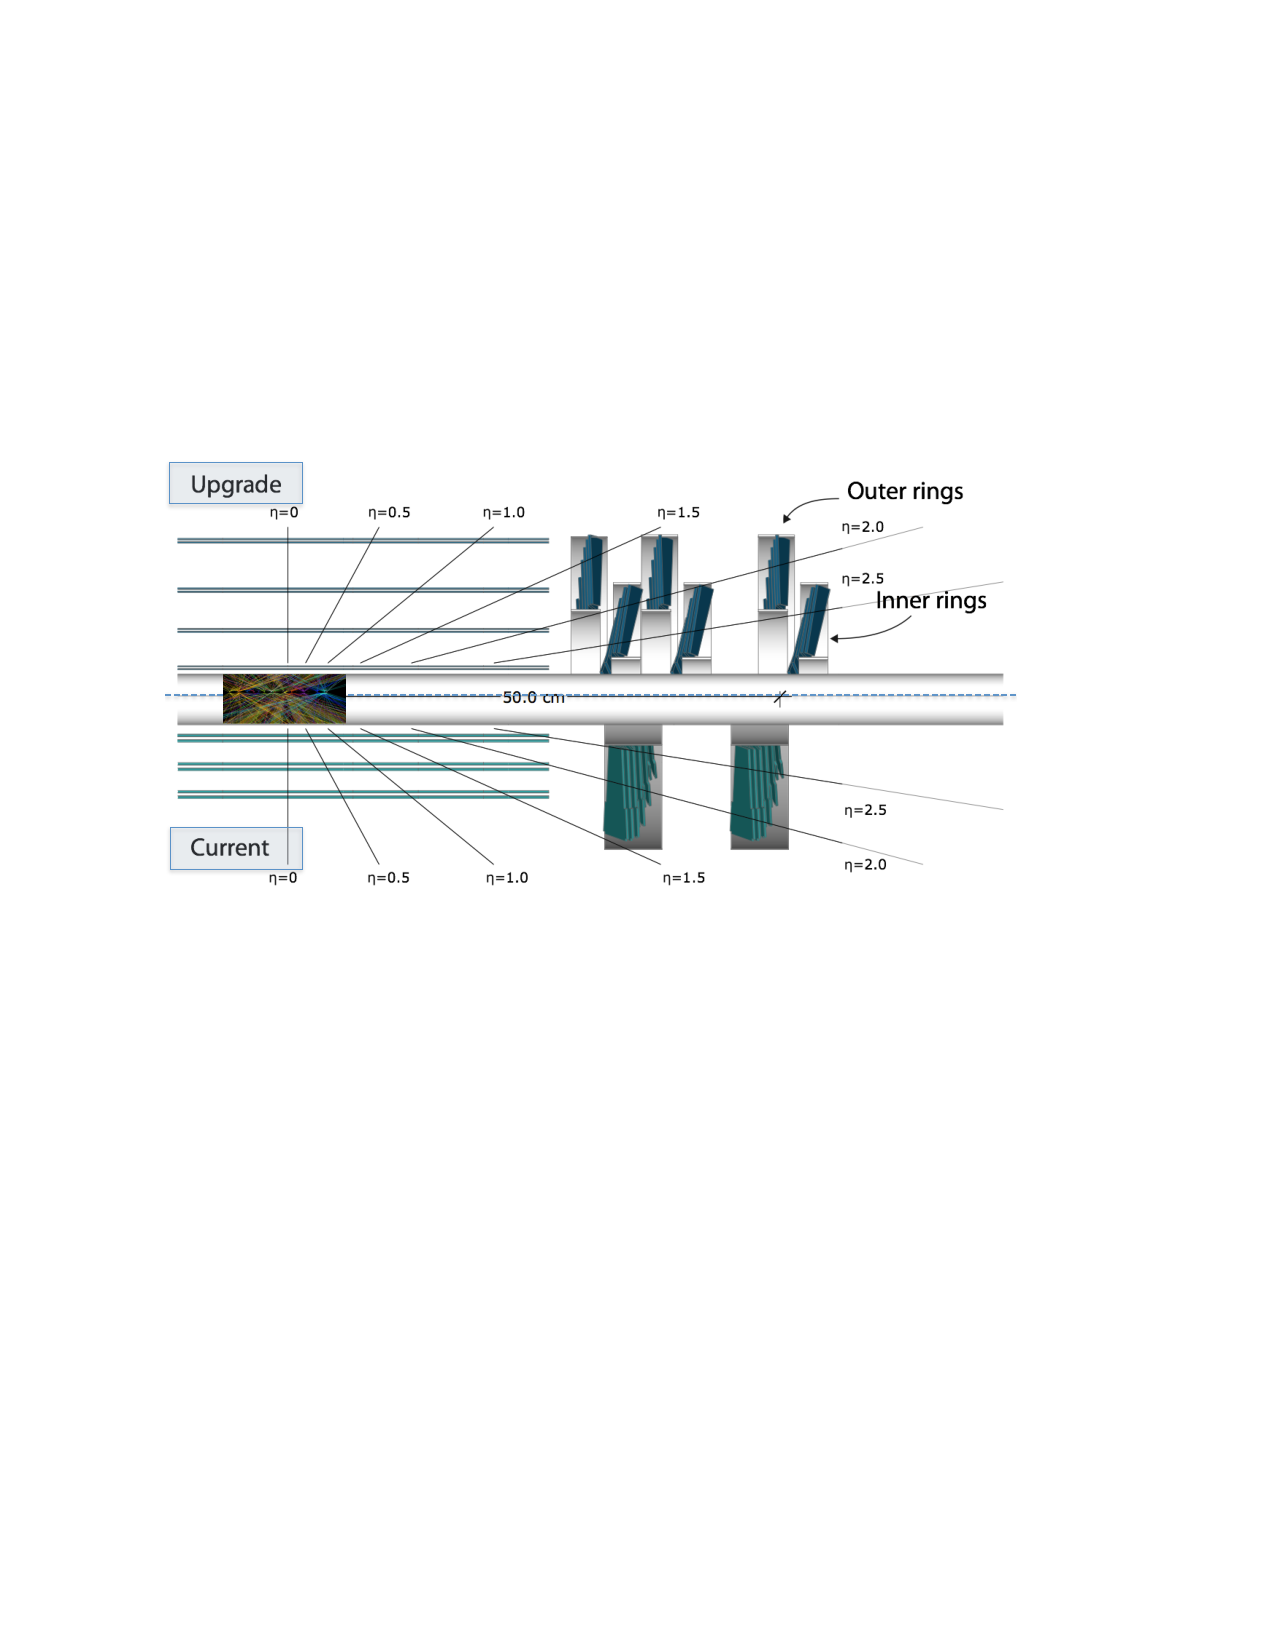
\includegraphics[width=0.43\textwidth]{figs/Phase-1-cropped}
\caption{\label{fig:phase1}Side-by-side comparison of the current CMS pixel detector and the Phase 1 Upgrade.  The upgraded detector must perform as well or better than the current detector at much higher instantaneous luminosity (up to $2 \times 10^{34}$~cm$^{-2}$s$^{-1}$) and remain performant up to 500/pb of integrated luminosity.  Additional pixel layers are added for more robust pattern recognition.}
\end{figure}
As shown in Figure~\ref{fig:phase1}, the upgraded Forward Pixel Detector will have three measurement layers (disks) per side, as opposed to the current two disks, complementing the extra fourth barrel layer. The UNL group helped with the overall design of this new detector and specifically with the module design.  To this end, Dominguez leveraged previous NSF awards and in particular an MRI to equip the clean room to produce the modules needed for the upgrade.  Dominguez and Meier  designed the custom tooling needed to do the pick and place assembly of the pixel modules.  These tools were all built by the UNL Instrumentation Shop.  The control software for the gantry was written by graduate students Jose Andres Monroy, Caleb Fangmeier and undergraduates Seth Kurfman and Davis Rempe.  Graduate student Joaquin Siado worked on the control and analysis code needed to run the test station that can readout four modules simultaneously while controlling the environmental conditions between room temperature and $-25^{\circ}$C.  Previous NSF grants and the  Cooperative Agreement supported this effort to be ready for the production of 550 modules at UNL.

Preliminary work has begun on the design of the next generation of detectors which will follow the Phase 1 Upgrade: the Phase 2 Upgrade.  This upgrade will be necessary at the end of the LHC Run~2, around 2024.  The entire CMS tracking system will be replaced to handle instantaneous and integrated luminosities about an order magnitude higher than those of Run~2.  Our group was one of the first to begin evaluating straw-man designs with simple simulations and parametric physics analyses.  Work done so far has shown that an extension of the forward pixel detector from psuedorapidities of 2.5 to 4.0 significantly extends the physics reach of CMS.  Dominguez has been asked to lead the U.S. efforts in the Phase 2 Forward Pixel Upgrade.
% KB -- let's argue this in the future work section, save a little space here.
%This work is challenging because it overlaps in time with the current run and the ongoing Phase-1 Upgrade.  
%More resources will be necessary in order to maintain this effort and leverage past success.
% AD -- I basically agree with Ken.  Currently, I think this is good here as an intro and segue to future work since this is in fact stuff we've already done, but we could condense it somehow if need be. We don't want unneeded repetition, but flow is important too.

In 2010-2011, Kravchenko, Butt, and undergraduates Pavel Patino and Gabriel Ayala  worked on studies for the track trigger that is envisioned for the Phase 2 upgrade of CMS. They studied several algorithms for fast jet reconstruction using information from the pixel detector that could be implemented within the Level 1 trigger time constraints, and implemented simple versions of these algorithms in an FPGA test board.

Snow continued his leadership of the 12-member CMS PhD Thesis Award Committee; he founded the program in 2000 and was appointed as chair of this committee in 2013~\cite{bib:thesisawardwebsite}.  Every year the committee reviews 15-20 theses, a number that has grown over time, and identifies one more award recipients each year.  This committee has also started to oversee a series of Named Lectures highlighting the contributions of outstanding young researchers to the experiment.

In 2014 Snow was elected as Deputy Chair of the U.S.~CMS Collaboration Board.  This has been an active period of time within U.S.~CMS governance, as new leadership of the Operations Program and Fermilab's LHC Physics Center needed to be appointed.  Snow was involved in those processes, along with many other search and election committees, as well as planning annual U.S. CMS collaboration meetings..

%XXX TODO: Greg please check if the Dzero results description is
%XXX complete, change it as needed, and once done please remove your name from
%XXX this comment.
\paragraph{DZERO} Contributions to the DZERO experiment continued after the Tevatron was shut down in September 2011 to complete the legacy of this fantastic physics program.

Former postdoc Michael Eads, on the faculty of Northern Illinois University since 2012, made significant contributions to DZERO throughout his seven years with the Nebraska group. He was convener of the New Phenomena physics group in 2010-12, a period of intense competition with the LHC. His own analysis work focused on searches for charged massive stable particles that would have the appearance of slow muons~\cite{bib:slowmuons}.  Former postdoc Ioannis Katsanos also searched for new phenomena, performing a search for a heavy gauge boson that decays to $e^+e^-$ pairs, setting limits in a variety of models~\cite{bib:IKheavyZ}.   Former graduate student Dale Johnston searched for the SM Higgs boson in $p\bar{p}$ collisions in the mode where it decays into a pair of $W$ bosons, the most sensitive channel at the Tevatron, for his PhD thesis~\cite{bib:dalethesis}.   Limits were set near twice the $W$ mass before first collisions at the LHC, and the analysis informed search strategies which led to the Higgs discovery.

The UNL group also made a major contribution to DZERO through operation of the luminosity monitors during the Tevatron run and the subsequent measurement of the integrated luminosity and its uncertainty. A number of DZERO measurements are limited by the integrated luminosity uncertainty.  Snow, Katsanos and former graduate student Kayle DeVaughan  all worked on this; Snow served as the co-convener of the DZERO luminosity group, with Katsanos succeeding him. Through much work, the luminosity uncertainty was reduced from 6.1\% to 4.2\%~\cite{bib:D0lumi}.

In addition, Bloom has chaired DZERO editorial boards supervising publications in top-quark physics. Among these have been measurements of the $t\bar{t}$ production forward-backward asymmetry that have been of great interest in the community~\cite{bib:D0afb}. Claes has served on an editorial board that has reviewed searches for new phenomena. Dominguez served on the editorial board for the measurements of $b$-jet identification. Finally, Snow has been responsible for the public tour area at the experiment, which was reconfigured as the experiment was decommissioned.

\paragraph{Astrophysics}

%XXX TODO Greg: please describe Auger results and papers (but not outreach, that's separate). But it is ok not to mention anything, because this section is already at the page limit.

Kravchenko has been working on several experiments on detection of ultra high energy
neutrinos of cosmic origin.  The RICE/NARC experiment, where Kravchenko was a key collaborator, finished in 2010. The final paper of the experiment was published in 2012~\cite{bib:RICE}. In 2011, Kravchenko joined the Askaryan Radio Array (ARA) experiment, the successor to RICE, based on the same detection idea and built at the same location. With a labor force  primarily of UNL undergraduates, Kravchenko worked on antenna array calibrations, development of reconstruction, and offline data processing of ARA. The experiment published several papers with contributions from Kravchenko's team \cite{bib:ARA}. He has also worked on the Telescope Array RAdar (TARA) experiment in Utah, which seeks to detect cosmic rays with a radar
technique~\cite{bib:CRADAR}.

\subsection{Broader Impact}

Since 2000, the Cosmic Ray Observatory Project (CROP)~\cite{bib:cropweb} has engaged teams of Nebraska high school science teachers and students in a large-scale study of cosmic ray air showers under the leadership of Claes and Snow. We now are working to bring the experience to the more remote rural schools in the state.  An ITEST-funded pilot project began with three rural and three Lincoln-area schools participating in CROP.  A series of Saturday workshops (three in Fall 2013, two in Spring 2014) trained teachers and students in the use of their own particle detectors. The first three-day workshops (one at the Educational Service Unit 10 offices for five rural area schools and one at UNL for six local schools) were held in Summer 2014. Following two fall workshops, school teams actively exercised the equipment in their own individually designed experiments, and reported on them in a Spring 2014 Saturday conference. Recruiting for additional schools began with hands-on workshop activities at the fall meetings of the Nebraska chapters of AAPT and NSTA. We secured Institutional Review Board approval from UNL and participating school districts, established a network of speakers from local tech industries (both urban and rural Nebraska) who conduct highly animated Q\&A sessions with students on STEM career opportunities, collected the baseline information for our evaluation, and established an on-demand solution center to promptly respond to student queries. Staff is being trained in the use of the CAMTASIA suite, the software used in creating our educational video training modules.

The Bilingual English Speaking Tutors (BEST) educational outreach program for Latino elementary school students is in its ninth year at Elliott Elementary School.  The program serves English language learner elementary school children and bilingual high school and UNL tutors who help the younger students twice a week for an hour after school on homework in the language most comfortable for both students.  Spanish- and Vietnamese-speaking tutors in the program come from Lincoln-area high schools.  English language learner teachers Jennifer Delka and Kara Hilzer coordinate the site at Elliott.  Last year the program expanded to a new elementary school, Rousseau, with Theresa Johnson as the lead coordinator. The BEST program is now fully developed and can be run by the coordinators without daily oversight by director Dominguez.

Bloom has continued as a U.S. LHC-sponsored blogger for the Quantum Diaries website~\cite{bib:bloomblog}.  In cooperation with ``The Big Bang Theory'' television program, he wrote a blog post~\cite{bib:TBBTQD} that was used as a major plot point in a February 2015 episode~\cite{bib:TBBTepisode}.  He continues to visit rural schools in Nebraska as time allows.  One recent visit was to Cambridge, NE, population 1047, where he met with all 350 students in the K-12 system.

%XXX TODO Ilya: add youtube links to LHC Season 2 videos and maybe US CMS videos
Gonzalez Suarez leads the UNL outreach effort at CERN. She has been an official CERN tour guide since 2011, conducting tours for the general public at multiple CERN experimental facilities, including the underground caverns of CMS and other experiments. Since 2014, Gonzalez Suarez has also guided virtual tours to the cavern of the CMS experiment for international audiences. In 2015 Gonzalez Suarez moderated several international masterclasses by the International Particle Physics Outreach Group from CERN. Gonzalez Suarez is also featured in the LHC Season 2 videos produced by CERN for the start of Run 2.

Kravchenko's work in RICE and ARA experiments, done entirely through the efforts of UNL undergraduate students, provides students with solid research experience, with two to four students involved at any given time over the last five years.  

%XXX TODO Greg: please review the Auger outreach paragraph below
Snow has continued as Auger Observatory Task Leader for Education and Outreach.  He oversees the Observatory's Visitor Center in Malarg\"{u}e, which has hosted more 90,000 visitors since it opened in 2001.  Snow is working with data acquisition experts on the experiment to broaden the dataset that is released to the public for educational purposes.  He has also organized five biennial Science Fairs that draw student teams from all over Mendoza Province in Argentina~\cite{bib:fairphotos}.  All of these efforts have been documented in presentations at the International Cosmic Ray Conferences~\cite{bib:ICRCoutreach}.

%XXX Greg: if you have any more events of this sort, please add. If not
%        please remove your name from this comment.
All faculty members continue to give presentations to public groups in Lincoln and elsewhere in Nebraska about the exciting science of particle physics. These have included over a dozen annual presentations of Claes's popular ``Comic Book Physics 101" series, YouTube videos inspired by these talks and produced by the American Chemical Society's ACS Reactions (featuring Claes as the consulting physics expert), and Claes's Spring 2015 public lecture targeting the general population of Lincoln, ``What the Heck is a Higgs Boson?" part of the UNL Chancellor's Distinguished Lecture Series.  Along with Claes, Snow is a member of UNL's Speakers Bureau, and has given presentations on the Higgs boson and ultra-high energy cosmic rays to civic groups, clubs and schools.

